\chapter{Background}
\label{chapter2}
In this chapter, we review some background knowledge that is going to be used in this dissertation. We begin with the introduction to probabilistic graphical models. Then a divergence measure is introduced. Common inference tasks and methods are discussed before the learning problems in probabilistic graphical models are reviewed, which are interpreted as minimization of the divergence measure.

\section{Graphical Models}
\label{chpt2:sec:graphical-models}
Graphical models provide a formal graph representation of statistical dependencies of complex problems or systems. The conditional independence of random variables can be conveniently encoded and analyzed by a graphical model. More importantly, query problems can be resolved by local message interactions of a graphical model in exact or approximate ways, which are usually infeasible to solve directly.

More formally, a graphical model is a graphical representation of a collection of random variables (along with their domains) where their statistical dependencies are encoded into a set of non-negative functions and the graphical structure. Let $\bm{x}= (x_1, x_2, \cdots, x_N)$ be a vector of random variables with $N$ as a positive integer, where an element variable $x_i$ can be either discrete or continuous random variable and takes values from its domain $\Xx_i$. Note that the domain of a random variable is not necessarily the same as that of another. With some abuse of notation, we might use $\bm{x}$ to denote its assignment when there is no cause of ambiguity in context. The joint probability distribution is described by its probability mass function (for discrete $\bm{x}$) or probability density function (for continuous $\bm{x}$), $p(\bm{x})=p(x_1, x_2, \cdots, x_N)$. We denote $\bm{\Xx} = \prod_{x=1}^{N} \Xx_i$ and then $\bm{x}\in \bm{\Xx}$. With an abuse of notation and concept, we say a probability distribution $p(\bm{x})$ in the sequel when it is clear in the context.

As motivated in Chapter~\ref{section1.1}, a graphical model can be directed or undirected. A directed graphical model is also known as a Bayesian network or generative model in the literature \cite[Chapter~8]{Bishop:2006:PRM:1162264}. We might use the names alternatively. The non-negative functions in graphical models encode the local compatibility of states of random variables. In directed graphical models, i.e., Bayesian networks, the local functions are conditional probability functions. The joint probability distribution is represented as the product of these conditional probability functions,
\begin{equation}
  p(\bm{x}) = \prod_{n=1}^{N}p(x_n| \Pp(x_n)),
\end{equation}
where $\Pp(\cdot)$ denotes the set of parent nodes in the directed graph. In a directed graphical model, the local functions, i.e., the conditional probability distributions $\{p(x_n| \Pp(x_n))\}$, are normalized and proper distributions. The directed graph of a directed graphical model or a Bayesian network is required to be an \textit{acyclic} graph. That is to say, starting from a node $1$ (associated with $x_1$) and following a directed path $x_1\rightarrow \cdots \rightarrow x_n$ along the directed edges of the graph, there is no path such that $n=1$. Sampling from the underlining distribution $p(\bm{x})$ of a directed graphical model is efficient. Due to acyclic property of directed graphical models, by the well-know \textit{ancestral sampling}, a sample $(x_1, x_2, \cdots, x_N)$ can be drawn sequentially via following the directed edges. In another word, $x_n$ is always sampled after $\Pp(x_n)$. This process might be viewed as the 'generative' process of signal $\bm{x}$, i.e., how $\bm{x}$ is generated from the graphical model.

A Bayesian network (generative model) is usually easier to interpret due to the fact that its local functions are conditional probabilities and it is natural to decompose the joint underlining distribution into conditional probability distributions. However, there are practical scenarios where interaction between two variables cannot be naturally described by impact with directionality, which may bring the difficulty of deciding the direction of an edge between them. Also, there are cases where a Bayesian network cannot encode all independence constraints of a distribution, which could be due to that certain structures are not appropriated by Bayesian networks (see \cite[Section~3.4.2]{koller2009pgm}). Therefore, an alternative representation method can be an undirected graphical model, i.e., a Markov random field (MRF). Under certain conditions, a Bayesian network can be perfectly represented by a Markov random field without loss of independence information by moralizing edges \cite[Section~4.5]{koller2009pgm}\cite[Section~8.3.4]{Bishop:2006:PRM:1162264}. Instead of conditional probability distributions, the local functions of MRF represents the compatibility of states of different variables, which are termed as \textit{potential factors}. Different from conditional probabilities in a Bayesian network, a potential factor in a MRF is not necessarily normalized (not necessary to sum up to one). We provide a toy example of MRFs as follows.
\begin{figure}[!t]
  % \captionsetup[subfigure]{justification=centering}
  \begin{subfigure}{.28\textwidth}
    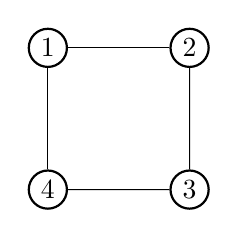
\begin{tikzpicture}
      \begin{scope}[scale=0.6]
        \tikzstyle{cnode} = [thick, draw=black, circle, inner sep = 2pt,  align=center]
        \node[cnode] (x1) at (0,0) {$1$};
        \node[cnode] (x2) at (3,0) {$2$};
        \node[cnode] (x3) at (3,-3) {$3$};
        \node[cnode] (x4) at (0,-3) {$4$};

        \draw[-] (x1) -- (x2);
        \draw[-] (x1) -- (x4);
        \draw[-] (x2) -- (x3);
        \draw[-] (x4) -- (x3);
      \end{scope}
    \end{tikzpicture}
  \end{subfigure}
  \begin{subfigure}{0.3\textwidth}
    \begin{tabular}{llc}
      \toprule
      $x_1$ & $x_2$ & $\phi(x_1, x_2)$ \\ %
      \midrule
      0  &  0  &  10 \\
      0  &  1  &  1 \\
      1  &  0  &  1 \\
      1  &  1  &  10\\
      \bottomrule
    \end{tabular}
  \end{subfigure}
  % \begin{subfigure}{0.05\textwidth}
  %   \centering
  %   \begin{tikzpicture}
  %     \node[] at (0,0) {$\cdots$};
  %   \end{tikzpicture}
  % \end{subfigure}
  \begin{subfigure}{0.3\textwidth}
    \begin{tabular}{llc}
      \toprule
      $x_2$ & $x_3$ & $\phi(x_2, x_3)$ \\
      \midrule
      0  &  0  &  5 \\
      0  &  1  &  3 \\
      1  &  0  &  3 \\
      1  &  1  &  5 \\
      \bottomrule
    \end{tabular}
  \end{subfigure}
  \begin{subfigure}{0.03\textwidth}
    \centering
    \begin{tikzpicture}
      \node[] at (0,0) {$\cdots$};
    \end{tikzpicture}
  \end{subfigure}
  \caption{A Markov random field with four binary nodes. Potential factors are represented by tables.}
  \label{chp2:fig:toy_mrf}
\end{figure}

\begin{example}\label{chpt2:mrf-3node-example}
  As shown in Figure~\ref{chp2:fig:toy_mrf}, the MRF encodes the dependencies of four random variables $x_1$, $x_2$, $x_3$, and $x_4$, where node $i$ is associated with variable $x_i$ and each has a binary domain, i.e., $\Xx_i = \{0,1\}$ for $i =1, 2, 3, 4$. Four potential factors of the MRF together define the joint distribution
  \begin{equation*}
    p(\bm{x}) = \frac{1}{Z} \phi_{1,2}(x_1, x_2) \phi_{2,3}(x_2, x_3) \phi_{1,4}(x_1, x_4)\phi_{3,4}(x_3, x_4)
  \end{equation*}
  where $Z = \sum_{x_1, x_2, x_3, x_4}\phi_{1,2}(x_1, x_2) \phi_{2,3}(x_2, x_3) \phi_{1,4}(x_1, x_4)\phi_{3,4}(x_3, x_4)$ normalizes the potential factors such that $p(\bm{x})$ is a proper distribution. The exemplified potential factors in Figure~\ref{chp2:fig:toy_mrf} demonstrate that it is more compatible or likely when $x_1$, $x_2$ and $x_3$ are in the same state (either $0$ or $1$) than when they are configured into different states.
\end{example}

From the above example to a formal statement, a MRF over random vector $\bm{x}$ can be represented by a undirected graph $\Gg(\Vv, \Ee)$, with each node $i \in \Vv$ is associated with a random variable $x_i$ and undirected edge set $\Ee \subset \Vv \times \Vv$. This MRF encodes a collection of distributions that factorize as
\begin{equation}\label{chp2:eq:mrf-definition}
  p(\bm{x};\bm{\theta}) = \frac{1}{Z(\bm{\theta})} \prod_{a \in \Ff} \phi_{a}(\bm{x}_{a};\bm{\theta}),
\end{equation}
where $\Ff$ is the set of indexes of potential factors, and each factor $\phi_{a}$ for $a\in \Ff$ is defined on subset of $\bm{x}$, i.e., $\phi_{a}: \Xx_{a} \rightarrow \RR^{+} \cup \{0\}$, where $\Xx_{a} = \prod_{i\in a}\Xx_i$ is the domain of potential factor $\phi_{a}$. The scope of factor $a$ is $\bm{x}_{a} = \left\{ x_i| i\in a \right\}$ where $i \in a$ stands for that the variable $x_i$ associated with node $i$ is an argument of potential factor $\phi_{a}$. In \eqref{chp2:eq:mrf-definition},
\begin{equation}
  Z(\bm{\theta}) = \sum_{\bm{x}} \prod_{a \in \Ff} \phi_{a}(\bm{x}_{a};\bm{\theta})
\end{equation}
is the \textit{partition function}. Obviously, the partition function normalizes the potential factors such that $p(\bm{x}; \bm{\theta})$ is a proper probability. $\bm{\theta}$ is the parameter set of potential factors $\left\{ \phi_a \right\}$.

\begin{remark}[On set $\Ff$ of potential factors]
In our definition in \eqref{chp2:eq:mrf-definition}, the set of potential factors, i.e., $\Ff$, is not required to be the set of all \textit{maximal cliques} of the graph $\Gg$. A clique of the graph $\Gg$ is a subset of nodes in $\Gg$, within which any two nodes are connected by an edge of $\Gg$. A maximal clique is a clique such that it is not possible to include any other nodes from $\Gg$ into the clique without it ceasing to be a clique. Note there is literature that defines MRF over maximal cliques \cite[Section~8.3.2]{Bishop:2006:PRM:1162264}. Actually, we can always reformulate \eqref{chp2:eq:mrf-definition} into factorization over maximal cliques by redefining a maximal clique as the product of potential factors (in $\Ff$) that are subsets of the maximal clique. Nevertheless, the definition in \eqref{chp2:eq:mrf-definition} without maximal clique requirement allows more flexibility of factorization and finer specification of potential factors. These properties may also benefit computations.
\end{remark}

\begin{remark}[Comparison of directed and undirected graphical models]
  We can compare directed and undirected graphical models with regard to the following aspects.
  \begin{itemize}
  \item \textit{Representation}: The structure and the parameterization in directed graphical models provide a natural representation for many types of real-world domains. For domains where interactions are naturally directional, directed graphical models can best manifest the abstraction and encode the dependencies. On the contrary, for domains where interactions are symmetrical without certain directionality, MRFs would be natural choices since forcing a directionality in these cases may cause an incomplete representation of dependencies. Furthermore, MRFs can be either cyclic or acyclic, which allows intuitive graphical representation with weaker constraints and gives the flexibility of graph structures.
  \item \textit{Local nonnegative functions}: The local functions are conditional probability functions in directed graphical models. In undirected graphical models, the local functions are potential factors that allow more flexible forms.
  \item \textit{Sampling}: Sampling is more straightforward within generative models (directed graphs) than that in MRFs.
  \item \textit{Normalization}: Since each local function is a conditional probability function in directed graphical models, the partition function for normalization is not needed. An MRF, in general, comes with a partition function, since potential factors are not necessarily normalized.
  \end{itemize}
\end{remark}

\begin{remark}[Graphical models with both directed and undirected edges]
  In the above discussions, we have presented both directed and undirected graphical models. In literature, a single graphical model may also encode both directed and undirected dependencies, i.e., there are both directed and undirected edges in its graph. Perhaps the most well-known models in this track are the \textit{conditional random fields} (CRFs). See \cite{charles2012crf} for more introduction.
\end{remark}


\subsection{An Alternative Representation}
\begin{figure}[!t]
  % \captionsetup[subfigure]{justification=centering}
  \begin{subfigure}{.33\textwidth}
    \centering
    \begin{tikzpicture}
      \begin{scope}[scale=0.7]
        \tikzstyle{cnode} = [thick, draw=black, circle, inner sep = 2pt,  align=center]
        \tikzstyle{nnode} = [thick, rectangle, rounded corners = 0pt,draw,inner sep = 5pt]
        \node[cnode] (x1) at (0,0) {$1$};
        \node[above=0.2mm of x1] {$x_1$};
        \node[cnode] (x2) at (3,0) {$2$};
        \node[above=0.2mm of x2] {$x_2$};
        \node[cnode] (x3) at (3,-3) {$3$};
        \node[below=0.2mm of x3] {$x_3$};
        \node[cnode] (x4) at (0,-3) {$4$};
        \node[below=0.2mm of x4] {$x_4$};

        
        \node[nnode] (f12) at (1.5, 0) {};
        \node[] at ($(f12) + (0,0.6)$) {$\phi_{1,2}$};
        \node[nnode] (f34) at (1.5, -3) {};
        \node[] at ($(f34) + (0,0.6)$) {$\phi_{3,4}$};
        
        \node[nnode] (f14) at (0, -1.5) {};
        \node[] at ($(f14) + (0.8,0)$) {$\phi_{1,4}$};
        \node[nnode] (f23) at (3, -1.5) {};
        \node[] at ($(f23) + (0.80,0)$) {$\phi_{2,3}$};
        \path[-, draw, thick]
        (x1) edge node {} (f12)
        (f12) edge node {} (x2)
        (x2) edge node {} (f23)
        (f23) edge node {} (x3)
        (x3) edge node {} (f34)
        (f34) edge node {} (x4)
        (x4) edge node {} (f14)
        (f14) edge node {} (x1)
        ;
      \end{scope}
    \end{tikzpicture}
    \caption{A factor graph representation.}
    \label{chpt2:fig:factor-graph-3node-example}
  \end{subfigure}
  \begin{subfigure}{.33\textwidth}
    \centering
    \begin{tikzpicture}
      \begin{scope}[scale=0.7]
        \tikzstyle{cnode} = [thick, draw=black, circle, inner sep = 2pt,  align=center]
        \tikzstyle{cfnode} = [thick, draw=black, fill=gray,circle, inner sep = 2pt,  align=center]
        \tikzstyle{nnode} = [thick, rectangle, rounded corners = 0pt,draw,inner sep = 5pt]

        \node[cnode] (x1) at (0,0) {$1$};
        \node[above=0.2mm of x1] {$x_1$};
        \node[cfnode] (x2) at (3,0) {$2$};
        \node[above =0.2mm of x2] {$x_2\!\!=\!\!1$};
        \node[cnode] (x3) at (3,-3) {$3$};
        \node[below=0.2mm of x3] {$x_3$};
        \node[cnode] (x4) at (0,-3) {$4$};
        \node[below=0.2mm of x4] {$x_4$};

        
        \node[nnode] (f12) at (1.5, 0) {};
        \node[] at ($(f12) + (0,0.6)$) {$\phi_{1,2}$};
        \node[nnode] (f34) at (1.5, -3) {};
        \node[] at ($(f34) + (0,0.6)$) {$\phi_{3,4}$};
        
        \node[nnode] (f14) at (0, -1.5) {};
        \node[] at ($(f14) + (0.8,0)$) {$\phi_{1,4}$};
        \node[nnode] (f23) at (3, -1.5) {};
        \node[] at ($(f23) + (0.80,0)$) {$\phi_{2,3}$};
        \path[-, draw, thick]
        (x1) edge node {} (f12)
        (f12) edge node {} (x2)
        (x2) edge node {} (f23)
        (f23) edge node {} (x3)
        (x3) edge node {} (f34)
        (f34) edge node {} (x4)
        (x4) edge node {} (f14)
        (f14) edge node {} (x1)
        ;
      \end{scope}
    \end{tikzpicture}
    \caption{Conditioning on $x_2=1$ in factor graph.}
    \label{chpt2:fig:factor-graph-3node-example-condition}
  \end{subfigure}
  \begin{subfigure}{.3\textwidth}
    \centering
    \begin{tikzpicture}
      \begin{scope}[scale=0.7]
        \tikzstyle{cnode} = [thick, draw=black, circle, inner sep = 2pt,  align=center]
        \tikzstyle{cfnode} = [thick, draw=black, fill=gray,circle, inner sep = 2pt,  align=center]
        \tikzstyle{nnode} = [thick, rectangle, rounded corners = 0pt,draw,inner sep = 5pt]


        \node[cnode] (x1) at (0,0) {$1$};
        \node[above=0.2mm of x1] {$x_1$};
        \node[cnode] (x3) at (3,-3) {$3$};
        \node[below=0.2mm of x3] {$x_3$};
        \node[cnode] (x4) at (0,-3) {$4$};
        \node[below=0.2mm of x4] {$x_4$};

        
        \node[nnode] (f12) at (1.5, 0) {};
        \node[] at ($(f12) + (1.2,0.6)$) {$\phi_{1,2}(x_1, x_2\!\!=\!\! 1)$};
        
        \node[nnode] (f34) at (1.5, -3) {};
        \node[] at ($(f34) + (0,0.6)$) {$\phi_{3,4}$};
        
        \node[nnode] (f14) at (0, -1.5) {};
        \node[] at ($(f14) + (0.8,0)$) {$\phi_{1,4}$};
        \node[nnode] (f23) at (3, -1.5) {};
        \node[] at ($(f23) + (-0.2,0.6)$) {$\phi_{2,3}(x_2\!\!=\!\! 1, x_3)$};

        \path[-, draw, thick]
        (x1) edge node {} (f12)

        (f23) edge node {} (x3)
        (x3) edge node {} (f34)
        (f34) edge node {} (x4)
        (x4) edge node {} (f14)
        (f14) edge node {} (x1)
        ;
      \end{scope}
    \end{tikzpicture}
    \caption{The reduced graph of Figure~\ref{chpt2:fig:factor-graph-3node-example-condition}}
    \label{chpt2:fig:factor-graph-3node-example-reduced}
  \end{subfigure}
  
  \caption{A Markov random field is represented by a factor graph in (a). Conditioning of the MRF in (b). The reduced MRF in (c).}
  \label{chp2:tab:toy-factor-graph}
\end{figure}

The previous graphical representations do not explicitly include the conditional probability functions or potential factors in their graphs. An alternative representation to a graphical model (undirected or directed) is \textit{factor graph} \cite{kschischang2001factor_graph},
which is a bipartite graph topology. In a factor graph, a potential factor or a conditional probability funciton is explicitly represented as a factor node, as the counterpart of the variable node associated with a random variable. We focus on the correspondence between a MRF and its factor graph here.
\begin{definition}\label{chpt2:def:factor-graph}
  A factor graph $\Gg_F$, is a bipartite graph that represents the factorization of \eqref{chp2:eq:mrf-definition}. A factor graph has two types of nodes: i) a variable node for each variable $x_i$; ii) a factor node for each potential function $\phi_{a}$. An edge is placed between a variable node $i$ and factor node $a$ if and only if $x_i$ is argument of $\phi_{a}$. We denote a factor graph by $\Gg_F(\Vv \cup \Ff, \Ee_F)$ with $\Vv$ as the set of variable nodes, $\Ff$ as the set of factor nodes, and $\Ee_F$ the set of undirected edges.
\end{definition}
\begin{example}
  Let us represent the Example~\ref{chpt2:mrf-3node-example} by a factor graph, which is shown in Figure~\ref{chpt2:fig:factor-graph-3node-example}. Different from the representation by $\Gg(\Vv, \Ee)$ in Figure~\ref{chp2:fig:toy_mrf}, factor nodes are explicitly represented by square nodes.
\end{example}


\subsection{Conditioning on Observations in MRFs}
It is not rare that a graphical model may contain observed variable. The node set of a MRF can be separated into a subset $\Vv_O$ of nodes that are associated with the observed variable $\bm{x}_O$, and a subset $\Vv_U$ of nodes associated with the unobserved variable $\bm{x}_U$. When an evidence is observed, its likelihood can be computed as
\begin{equation}
  p(\bm{x}_O;\bm{\theta}) = \sum_{\bm{x}_U} p(\bm{x};\bm{\theta}) =\sum_{\bm{x}_U}\frac{\tilde{p}(\bm{x}; \bm{\theta})}{Z(\bm{\theta})} = \frac{Z(\bm{x}_O,\bm{\theta})}{Z(\bm{\theta})},
\end{equation}
where 
\begin{align}
  \tilde{p}(\bm{x}; \bm{\theta}) &= \prod_{a \in \Ff} \phi_{a}(\bm{x}_{a};\bm{\theta}), \nonumber \\
  Z(\bm{x}_O, \bm{\theta}) &= \sum_{\bm{x}_U} \tilde{p}(\bm{x}; \bm{\theta}), \nonumber \\
  Z(\bm{\theta}) &= \sum_{\bm{x}_O}\sum_{\bm{x}_U} \tilde{p}(\bm{x}; \bm{\theta}).
\end{align}
This means that the likelihood of an (partial) evidence can be computed by partition function and sub-partition functions. As shall be seen in Part~\ref{part:learning}, this likelihood function, or its approximation will be used for model learning.

 When an evidence $\bm{e}_O$ (a sample instance of $\bm{x}_O$) is observed, the conditional probability can be written as
\begin{equation}\label{chpt2:eq:mrf-condtioning}
  p(\bm{x}_U|\bm{x}_O=\bm{e}_O;\bm{\theta}) = \frac{\tilde{p}(\bm{x}_U, \bm{x}_O = \bm{e}_O; \bm{\theta})}{\sum_{\bm{x}_U}\tilde{p}(\bm{x}_U, \bm{x}_O = \bm{e}_O; \bm{\theta})} \propto \tilde{p}(\bm{x}_U, \bm{x}_O = \bm{e}_O; \bm{\theta}),
\end{equation}
where $\propto$ stands for proportional to. Note that \eqref{chpt2:eq:mrf-condtioning} shows an interesting phenomenon for MRF including evidence. It can be understood as clamping nodes in $\Vv_O$ of the MRF to configuration $\bm{e}_O$, i.e., the domain of $\bm{x}_O$ becomes a set containing only one instance $\bm{e}_O$. For instance, an example of conditioning on a variable node for Example~\ref{chpt2:mrf-3node-example} is shown in Figure~\ref{chpt2:fig:factor-graph-3node-example-condition}, where node $2$ is clamped to evidence $x_2=1$.



In addition to the above intuitions, conditioning can also be understood as a process of reducing the graph of an MRF. When an MRF is conditioned on $\bm{x}_O$, the variables nodes of set $\Vv_O$ are removed from $\Gg$, along with their edges. The potential factors with regard to $\Vv_U$ are modified accordingly \cite[Chapter~4.2.3]{koller2009pgm}. For instance,
the graph including evidence node $2$ in Figure~\ref{chpt2:fig:factor-graph-3node-example-condition} can be further reduced into a Figure~\ref{chpt2:fig:factor-graph-3node-example-reduced}. Then any inference applicable to an MRF applies to the MRF with nodes clamped as well. An MRF with several nodes clamped to some evidence can be seen either as a manipulation of its domain or the graph itself.


It can be seen that the MRF framework is capable of handling evidence and conditioning as well. We will come back to this topic in Part~\ref{part:learning}.

\section{Divergence}\label{chpt2:sec:devergence}
Before we get into further discussions about inference and learning, we first introduce the concept of \textit{divergence} measures since principles of both learning and inference are closely related to divergence measures.
A divergence measure plays a fundamental role when we try to use a probability distribution (over discrete or continue variable)  $q$ to approximate another probability distribution $p$. A divergence measure is used to formally quantify how much information is lost when $p$ is represented by $q$. Denote $\PP$ as the space of measures $p$ and $q$, i.e., $p, q \in \PP$.
\begin{definition}
  Given the space $\PP$ of probability distributions for a random variable $\bm{x}$, a divergence on this space is defined as a function $D(p\|q): \PP \times \PP \rightarrow \RR^{+}\cup \{0\}$ such that $D(p\|q) \geq 0$ for all $p, q \in \PP$ and $D(p\|q)=0$ if and only if $p=q$.
\end{definition}

Here we introduce the classic \textit{Kullback-Leibler divergence} \cite{kullback1959, kullback1951}, KL divergence for short, which is one of the most widely used divergence measures in machine learning, statistics and information theory.
\begin{definition}
  The Kullback-Leibler (KL) divergence on $\PP$ is defined as a function $KL(\cdot \| \cdot): \PP \times \PP \rightarrow \RR^{+} \cup {0}$ with the following form
  \begin{equation}\label{chpt2:def:kl-divergence}
    \mathrm{KL}(p\|q) = \sum_{\bm{x}}p(\bm{x}) \log{\frac{p(\bm{x})}{q(\bm{x})}},
  \end{equation}
  where $\log$ is the natural logarithm. Note that the sum in \eqref{chpt2:def:kl-divergence} should be replaced by an intergral when $p$ and $q$ are probability density functions.
\end{definition}


The KL divergence is not symmetric. In other words, there is no equivalence between $\mathrm{KL}(p\|q)$ and $\mathrm{KL}(q\|p)$ in general. A symmetric divergence that generalizes the KL divergence will be introduced in Section~\ref{chpt3:sec:alpha-divergence}. Furthermore, an extra metric that is used to compare distributions, i.e., optimal transport, will be introduced in Section~\ref{chpt8:sec:ot}.



\section{Inference Tasks}


Given a probability distribution $p(\bm{x})$ as the underlying distribution of a graphical model, inference in general can be divided into four kinds of tasks, as explained in Chapter~\ref{chpt1:sec:scope-outline}. Our work in this dissertation is closely involved with the following problems in MRFs
\begin{itemize}
\item computing the likelihood of observed data or unobserved random variables;
\item computing the marginal distribution over a particular subset of nodes, i.e., $p(\bm{x}_A)$ for $A \subset \Vv$. Note that a single-node marginal distribution $p(x_i)$ also belongs to this case;
\item computing the conditional distribution of a subset of nodes given the configuration of another subset of nodes, i.e., $p(\bm{x}_A| \bm{x}_B)$ for $A, B \in \Vv$ and $A \cap B = \emptyset$.
\end{itemize}
The above tasks are also closely related with the inference of the partition function, i.e.,
\begin{itemize}
\item computation of $Z(\bm{\theta}) = \sum_{\bm{x}} \prod_{a \in \Ff} \phi_{a}(\bm{x}_{a};\bm{\theta})$, or sub-partition functions.
\end{itemize}

In the following section, we introduce the methods for the above tasks at a high-level.

\section{Exact Inference}
\label{chpt2:sec:inference-mp}
In this section, we briefly treat the exact inference of graphical models. Please see \cite{Bishop:2006:PRM:1162264, koller2009pgm, yedida2005constucting, yedidia2003understanding} for detailed discussions. In order to compute a marginal probability, we need to sum or integrate the joint probability distribution over some variables. This operation can be performed as a sequence of operations by a pre-defined ordering of the variables. Since the underlying distribution of a graphic model (directed or undirected) is a product of factors, the sequence or order can be chosen in a way that facilitates the sum or integral operations. Thus the computation of the marginal probability is up to choosing a specific ordering of remaining variables to eliminate (sum or integrate out) repeatedly. This brings the very fundamental exact inference method, \textit{variable elimination}.

When we want to ask multiple queries (marginal probabilities) on a graphical model, we repetitively call the variable elimination method for each query until all queries are answered. The \textit{sum-product} algorithm is more efficient for this case. It is a \textit{message passing} algorithm that operates on graphical models. More importantly, the intermediate results, the messages, are shared in all computations. Thus one call of this message passing algorithm returns answers to multiple queries. The sum-product algorithm, also known as \textit{belief propagation}, has an iterative message update rule. A message update step from a factor $a$ to its neighboring variable node $i$ is 
\begin{equation}\label{chpt2:eq:loopy-bp}
  m_{a\rightarrow i}(x_i) \propto \sum_{\bm{x}_{a} \backslash x_i}
  \phi_{a}(\bm{x}_{a}) \prod_{j \in a \backslash i} \prod_{a^{\prime} \in \mathrm{ne}_j
    \backslash a} m_{a^{\prime}\rightarrow j}(x_j),
\end{equation}
where $a^\prime, a \in \Ff$ and $\mathrm{ne}_i = \left\{ a | i \in a, a \in \Ff \right\}$ denotes the neighboring factors of the variable node $i$. The left-hand-side of $\propto$ is the updated message and the right-hand-side of $\propto$ is a function of factors and old messages in \eqref{chpt2:eq:loopy-bp}. The marginal for $x_i$ is simply $p(x_i)\propto\prod_{a\in\mathrm{ne}_i}m_{a\rightarrow i}(x_i)$ after all messages have been updated accordingly. For a tree-structured graph, the message passing rule in \eqref{chpt2:eq:loopy-bp} with pre-defined ordering of sequential updates gives exact marginals.

However, when a graphical model is not tree-structured, the above methods can not give exact inference. If exact inference is still desired here, one may consider converting the graph of the graphical model into a clique tree, an acyclic graph whose nodes are maximal cliques, and apply the \textit{junction tree} algorithm.

It is known that the computational complexity of the junction tree method grows exponentially in the size of the maximal clique. Therefore, for certain classes of graphs, exact inference is feasible by using the methods mentioned above. On the other hand, there are many graphical models where exact inference is too expensive in computation or simply prohibitive. We need to turn to approximate inference to cope with such models.


\section{Variational Inference}
\label{chpt2:sec:variational-inference}

In solving inference tasks with approximation, one important technique is based on a variational approach. With $p(\bm{x};\bm{\theta})$ as the underlying probability distribution of a graphical model, direct inference with $p(\bm{x}; \bm{\theta})$ is often unfeasible due to the system represented by the graphical model being too large or complex. It can also be the case that even we know the form of $p(\bm{x}; \bm{\theta})$, the computation in inference tasks can be prohibitive. In variational approaches, a 'trial' probability distribution $b(\bm{x})$ is introduced to approximate $p(\bm{x};\bm{\theta})$. The trial distribution should be intuitively simpler than $p(\bm{x}; \bm{\theta})$. \textit{Variational free energy} \cite{opper2001advanced} is a quantity used to find such a approximation. The variational free energy is defined by
\begin{align}\label{chpt2:eq:variational-free-energy}
  F_V(b) & = \mathrm{KL}(b( \bm{x}) || p(\bm{x}; \bm{\theta})) - \log{Z(\bm{\theta})} \nonumber \\
         &= \sum_{\bm{x}}b(\bm{x}) \log{\frac{b(\bm{x})}{{p}(\bm{x}; \bm{\theta})}} - \log{Z(\bm{\theta})} \nonumber \\
         & = \sum_{\bm{x}}b(\bm{x}) \log{\frac{b(\bm{x})}{\tilde{p}(\bm{x}; \bm{\theta})}},
\end{align}
where $\tilde{p}(\bm{x}; \bm{\theta}) =  \prod_{a \in \Ff} \phi_{a}(\bm{x}_{a}; \bm{\theta})$. Since $\mathrm{KL}(b(\bm{x})\|p(\bm{x};\bm{\theta}))$ is always non-negative and is zero if and only if $b(\bm{x}) = p(\bm{x};\bm{\theta})$, we have $F_V(b) \geq - \log{Z(\bm{\theta})}$, with equality when $b(\bm{x}) = p(\bm{x};\bm{\theta})$.

\begin{remark}[Interpretation of variational free energy]
  Note from \eqref{chpt2:eq:variational-free-energy}, the minimization with regard to $b$ of variational free energy is equivalent to the divergence minimization, i.e., $\mathrm{KL}(b( \bm{x}) || p(\bm{x}; \bm{\theta}))$, since $\log{Z(\bm{\theta})}$ does not depend on $b$. By observing $F_V(b) = \sum_{\bm{x}}b(\bm{x}) \log{\frac{b(\bm{x})}{\tilde{p}(\bm{x}; \bm{\theta})}}$, the free energy minimization guides the choice of $b$ such that $b$ is close to an unnormalized measure $\tilde{p}(\bm{x}; \bm{\theta})$ in its space.

  Another benefit of \eqref{chpt2:eq:variational-free-energy} is that we are able to approximate $p(\bm{x}; \bm{\theta})$ without inference of the true marginal distributions $\{p(\bm{x}_{a};\bm{\theta}), a \in \Ff\}$. Since $\log\tilde{p}(\bm{x}; \bm{\theta})$ can be formulated as sum of log-potential-factors that are all local functions, the computation of $F_V(v)$ can be done by inference of marginals $\left\{ b_{a}(\bm{x}_{a}), a \in \Ff \right\}$ of the approximate distribution, which are tractable.
\end{remark}

\begin{remark}[Discussion]
  Since we are essentially approximating distribution $p$ by a distribution $b$, can we minimize $\mathrm{KL}(p(\bm{x}, \bm{\theta})\|b(\bm{x}))$ instead?

  It might be feasible by instinct. But a further check would reveal its infeasibility. The $\mathrm{KL}(p(\bm{x}; \bm{\theta})\|b(\bm{x}))$ would inevitable require the marginals of $p$ and therefore requires the exact inference in $p$, which are what we are trying to avoid. But it does not mean this divergence is useless. As shall be seen in Section~\ref{chpt2:sec:learning-principles}, this type of divergence measure is what we need in model learning.
\end{remark}



\subsection{Variational Free Energy and Mean Field}

Mean field method, similar to the sum-product algorithm in Section~\ref{chpt2:sec:inference-mp}, is an iterative message passing approach. 
The message update rule of mean field algorithm is described as follows.
\begin{equation}\label{chpt2:eq:mf-update}
  \log{b_i(x_i)} \propto \sum_{a \in \mathrm{ne}_i} \sum_{\bm{x}_{a} \backslash x_i} \prod_{j\in {a}\backslash i} b_j(x_j)\log{\phi_{a}}(\bm{x}_{a};\bm{\theta}_{a}).
\end{equation}
The algorithm does iterative updates of the belief on each node of the graphical model. An update step for node $i$ uses its neightbors' old  beliefs  $\left\{ b_j(x_j), j\in {a}\backslash i, a \in \mathrm{ne}_i \right\}$ and factors to assign new belief $b_i(x_i)$. After the iterative algorithm converges, the approximation to marginal $p(x_i)$ is $b_i(x_i)$.


The intuition of mean field algorithm can be given by the variational free energy defined in \eqref{chpt2:eq:variational-free-energy}. In fact, mean field approach uses the fully-factorized distribution,
\begin{equation}\label{eq:mf-factorization}
  b_{MF}(\bm{x}) = \prod_{i=1}^{N}b_i(x_i),
\end{equation}
to approximate the joint distribution $p(\bm{x};\bm{\theta})$. The update rule \eqref{chpt2:eq:mf-update} can be obtained by minimizing the 'difference' between the fully-factorized distribution and $p(\bm{x};\bm{\theta})$, i.e., the variational free energy \eqref{chpt2:eq:variational-free-energy}. Specifically,
substituting \eqref{eq:mf-factorization} into the variational free energy \eqref{chpt2:eq:variational-free-energy} gives
\begin{align}
  F_{MF}(b) =  - \sum_{a \in \Ff}\sum_{\bm{x}_{a}} \prod_{i\in a}b_i(x_i)\log{\phi_{a}(\bm{x}_{a};\bm{\theta})}
   + \sum_{i \in \Vv} \sum_{x_i} b_i(x_i) \log{b_i(x_i)}.
\end{align}
Minimizing $F_{MF}(b)$ over $\left\{ b_i \right\}$ would give us the mean field update rule \eqref{chpt2:eq:mf-update}.

\subsection{Bethe Free Energy and (Loopy) Belief Propagation}

We described the sum-product algorithm (belief propagation) for exact inference in tree-structured graphs in Section~\ref{chpt2:sec:inference-mp}. For graphical models with the presence of cycles or loops, we can still apply the sum-product algorithm as if there was no loop. This is known as the loopy belief propagation (loopy BP). Of course, the inference results are no longer exact. But loopy BP still works well in many practical cases.

Now we give the intuition of loopy BP from the perspective of free energy minimization, which comes with the name of Bethe approximation in literature.
Different from the mean field approximation, Bethe approximation also includes the non-single-node beliefs $\{b_{a}(\bm{x}_{a})\}$ apart from the single-node beliefs $\{b_i(x_i)\}$\cite{yedidia2003understanding}. In this case, the Bethe free energy is given by
\begin{align}\label{chpt2:bethe-free-energy}
  F_{Bethe}(b) = \sum_{a\in \Ff} \sum_{\bm{x}_{a}}
  b_{a}(\bm{x}_{a})\log{\frac{b_{a}(\bm{x}_{a})}{\phi_{a}(\bm{x}_{a})}
  } -  \sum_{i=1}^{N} (|\mathrm{ne}_i| - 1) \sum_{x_i} b_i(x_i) \log{b_i(x_i)},
\end{align}
where $|\cdot|$ stands for cardinality.
Due to the  non-single-node beliefs, there are consistency constrains $\sum_{\bm{x}_{a}} b_{a}(\bm{x}_{a}) = \sum_{ x_i} b_i({x}_i) =1$, $\forall~ i \in a$ to obey. Then, solving the Bethe free energy minimization problem
\begin{align}
  \min_{\{b_{a}(\bm{x}_{a})\}, \{b_i(x_i)\}}& F_{Bethe}(b) \nonumber \\
  \mathrm{s.t.}~~ & \sum_{\bm{x}_{a} \backslash x_i} b_{a}(\bm{x}_{a})  =
                    b_i(x_i), \nonumber \\
                                                      & \sum_{\bm{x}_{a}} b_{a}(\bm{x}_{a}) = \sum_{ x_i} b_i({x}_i) =1,
                                                        \nonumber \\
                                                      &  0 \leq b_i(x_i) \leq 1,  \nonumber \\
                                                      & i \in \Vv , a \in \Ff,
\end{align}
where $\Vv$ and $\Ff$ are the set of variable nodes and the set of
factor nodes in factor graph as defined in
Definition~\ref{chpt2:def:factor-graph}, gives the (loopy) BP message passing rule that has the same formula as in \eqref{chpt2:eq:loopy-bp}.

These variational approaches will be further discussed and compared in Chapter~\ref{chapter3} and \ref{chapter4} of Part~\ref{part:inference}.

\section{Learning Principles}
\label{chpt2:sec:learning-principles}
We have touched the learning topic in Chapter~\ref{chapter1}, which is to find the 'best' probability distribution $p(\bm{x}; \bm{\theta})$ in its space $\PP$. To make the discussion more concrete, we assume the domain is governed by an underlying distribution $p^{\ast}$ that is induced by a (directed or undirected) graphical model, $\Mm^{\ast} = \left\{ \Kk^{\ast}, \bm{\theta}^{\ast} \right\}$ with $\Kk^{\ast}$ representing its structure and $\bm{\theta}^{\ast}$ representing its parameter. Here we discuss about \textit{model learning} (parameter learning only). For notation simplicity, we use $p^{\ast}(\bm{x})$ to denote this distribution. We are given a dataset $\Dd = \{\bm{x}^{1}, \bm{x}^{2}, \cdots, \bm{x}^{M}\}$. Following the standard assumption, these sample instances are \textit{independent and identically distributed (i.i.d.)} according to $p^{\ast}(\bm{x})$. The task is then to use the information from the dataset to learn a distribution $p(\bm{x};\bm{\theta})$ within its space $\PP$, since the governing distribution $p^{\ast}(\bm{x})$ is not known.

The problem of learning a distribution in $\PP$ to approximate $p^{\ast}$ can be formulated as density estimation. With the concept of KL divergence in Section~\ref{chpt2:sec:devergence}, learning of $p(\bm{x};\bm{\theta})$ can be formulated as minimizing the KL divergence
\begin{align}\label{chpt2:sec:mle-as-min-kl}
  &\mathrm{KL}(p^{\ast}(\bm{x})\|p(\bm{x}; \bm{\theta})) \nonumber \\
  =& \EE_{p^{\ast}(\bm{x})}\left[ \log{\frac{p^{\ast}(\bm{x})}{p(\bm{x}; \bm{\theta})}} \right] \nonumber \\
  =& - H(p^{\ast}) - \EE_{p^{\ast}(\bm{x})}\left[ \log{{p(\bm{x}; \bm{\theta})}} \right],
\end{align}
where $H(p^{\ast})$ is the entropy of $p^{\ast}$.
Due to the property of divergence, the KL divergence in \eqref{chpt2:sec:mle-as-min-kl} is zero if and only if $p(\bm{x};\bm{\theta})=p^{\ast}(\bm{x})$. The last line of \eqref{chpt2:sec:mle-as-min-kl} shows that the negative entropy term does not depend on $p(\bm{x}; \bm{\theta})$. Thus we can just focus on the negative expectation term $-\EE_{\bm{x} \sim p^{\ast}}\left[ \log{{p(\bm{x}; \bm{\theta})}} \right]$, which is the \textit{cross entropy}. Therefore, we can just use the cross entropy to do model learning.

Note that although we can use the cross entropy for the model learning task and for even model comparison (comparing a trained model with another one), we lose the information of how close a trained model is to $p^{\ast}$. This is due to the omission of $H(p^{\ast})$, which is not available.

Since it is not possible to know $p^{\ast}$ (otherwise we do not need to learn it), the (negative) cross entropy is approximated by sample instances of $p^{\ast}$,
\begin{equation}
  \Ll(\Dd; \bm{\theta}) = \frac{1}{\abs{\Dd}}\sum_{\bm{x}\in \Dd}\log{p(\bm{x};\bm{\theta})},
\end{equation}
and
\begin{equation}
  \EE_{p^{\ast}(\bm{x})}\left[ \log{{p(\bm{x}; \bm{\theta})}} \right] \approx \Ll(\Dd; \bm{\theta}).
\end{equation}


The log-likelihood $\Ll(\Dd; \bm{\theta})$ is one of the most widely used loss functions for model learning. However, $\Ll(\Dd; \bm{\theta})$ is not always a feasible loss to compute (see Chapter~\ref{chpt5:undirecteLearning} for more analyses) since
\begin{itemize}
\item it is often that exact computation of $p(\bm{x};\bm{\theta})$ is not possible; or
\item there are some elements of $\bm{x}$ which are not observable (hidden or latent variables).
\end{itemize}
For the first case, the typical treatment is to approximate the exact log-likelihood. This is done via approximation by employing inference methods or   making simplified assumptions on dependency structure of the graphical model of $p(\bm{x})$. Then, optimization is carried out with regard to the approximated log-likelihood. These methods include surrogate likelihood \cite{wainwright06estimating, lu2019blockBP}, pseudo-likelihood\cite{qu2019gmnn, lazarogredilla2019learning}, piecewise likelihood \cite{sutton2012piecewise, lin_2016_CVPR}, saddle-point approximation \cite{srikumar-etal-2012-amortizing, NIPS2019_9687}.

Apart from the above case where all variables are observable, the partial observed models, the latent variable case, are equally import in inference and learning with uncertainty. This class of models includes (but is not limited to) classic Gaussian mixture models (GMMs) and hidden Markov models (HMMs). There are latent variables because:
\begin{itemize}
\item Use of abstract variables to model the generative process (usually a directed graph) of observation data, such as HMMs.
\item A practical true attribute of an object may be difficult or impossible to measure exactly. For instance, disease infection can only be diagnosed via the relevant symptoms, see e.g., Example~\ref{example-corona}. In the position tracking of a car with noisy sensors, the true position of the car might only be inferred via noisy data of sensors.
\item No measurement on an attribute of an object of interest is made. For instance, the velocity sensor in the car tracking example might not be stable and might fail from time to time.
\end{itemize}
In general, latent variables are commonly used to deal with partial observation problems, data clustering, data manipulation, etc. Let us denote the observable variable and latent variable by $\bm{x}_O$ and $\bm{x}_U$, respectively. We can see that the log-likelihood $p(\bm{x}_O, \bm{x}_U; \bm{\theta})$ is not available anymore as it is in the fully-observed case. To deal with the latent variables, we can try to optimize the partial log-likelihood
\begin{align}
  l(\bm{x}_O; \bm{\theta}) =& \log{p(\bm{x}_O; \bm{\theta})} \nonumber \\  
  = & \EE_{q(\bm{x}_U|\bm{x}_O)}\left[ \log{\frac{q(\bm{x}_U|\bm{x}_O)}{p(\bm{x}_U|\bm{x}_O;\bm{\theta})} \cdot \frac{p(\bm{x}_U,\bm{x}_O;\bm{\theta})}{q(\bm{x}_U|\bm{x}_O)}} \right] \nonumber \\
  = & \mathrm{KL}(q(\bm{x}_U|\bm{x}_O)\|p(\bm{x}_U|\bm{x}_O;\bm{\theta})) + F(q, \bm{\theta})
\end{align}
with
\begin{equation}\label{chpt2:eq:llk-lower-bound}
  F(q, \bm{\theta}) = \EE_{q(\bm{x}_U|\bm{x}_O)}\left[ \log{p(\bm{x}_U,\bm{x}_O;\bm{\theta})} \right] + H(q(\bm{x}_U|\bm{x}_O))
\end{equation}
where $H(q(\bm{x}_U|\bm{x}_O))$ is the entropy of $q(\bm{x}_U|\bm{x}_O)$, and $q$ can be any distribution over $\bm{x}_U$. Due to the non-negative property of KL divergence, we have
\begin{equation}
  l(\bm{x}_O; \bm{\theta}) \geq F(q, \bm{\theta}),
\end{equation}
with equality when $q(\bm{x}_U|\bm{x}_O) = p(\bm{x}_U|\bm{x}_O; \bm{\theta})$. $F(q, \bm{\theta})$ is also called \textit{variational lower bound}.

One of the most widely used methods in learning with latent variable is \textit{expectation maximization (EM)} \cite{dempster1977maximum}. In the EM method, the posterior of $\bm{x}_U$ is computed exactly from $p$, $q(\bm{x}_U|\bm{x}_O) = \argmax_{q}{F(q, \bm{\theta})} = p(\bm{x}_U|\bm{x}_O; \bm{\theta})$, which is the optimal solution to $q$. Then the parameter $\bm{\theta}$ of $p$ is optimized. The two steps are optimized iteratively. The detailed treatment can be found in Part~\ref{part:learning}

In cases where the posterior of $\bm{x}_U$ is not feasible to compute, the variational EM \cite[Section~6.2.2]{wainwright2008graphical} or Monte Carlo EM (need sampling technique) \cite{neath2012convergence} can be applied. There are also neural network based methods with Monte Carlo estimator to cope with the latent variable problems, see e.g., \cite{DBLP:journals/corr/KingmaW13, kuleshov2017neural_variational, lazarogredilla2019learning, goodfellow2014gan}.


In the above discussion, we have assumed that the model's distribution $q$ is explicitly defined, i.e., the distribution (along with its density function or mass function) is available. 

In an alternative track, deep generative models have gained growing popularity in literature and can be applied to different areas such as high-dimensional data representation, reinforcement learning, and semi-supervised learning, because of its efficient sampling of multi-mode distributions \cite{2017arXiv170100160G}. A generator in a deep generative model induces a distribution that can either be an explicit or implicit distribution. The former problem dates back to \cite{deco1995high-order} and receives more attention in recent years with latest work such as variational autoencoder \cite{DBLP:journals/corr/KingmaW13}, normalizing flows \cite{2016arXiv160508803D, 2018arXiv180703039K} and neural ordinary difference equations \cite{ricky2018ODE}. The training of explicit models is based on the maximum likelihood principle or variational likelihood bound. Chapter~\ref{chpt6:em-flow} and \ref{chpt7:genhmm} will give detailed treatment with modeling and learning with normalizing flows. Chapter~\ref{chapter9} will further discuss the implicit deep generative models and their learning.

The latter case brings an implicit distribution, where the maximum likelihood principle is not applicable anymore. In this case, a state-of-art method is the generative adversarial model that employs a discriminator to play the role of divergence measure \cite{goodfellow2014gan, 2017arXiv170104862A, NIPS2016_6125}, which is essentially explained by a process of the minimization of the Jensen-Shannon divergence. Additionally, other sample-test based distances are employed as alternative methods for implicit model learning. Among this family, optimal transport is receiving more attention in recent years \cite{santambrogio2015optimal, 2013arXiv1306.0895C} in this track, which has also been applied for training of Boltzmann machine \cite{NIPS2016_6248} auto-encoders\cite{2017arXiv171101558T} and generative adversarial networks \cite{2017arXiv170107875A}. We discuss this further in Chapter~\ref{chapter9}.



%%% Local Variables:
%%% mode: latex
%%% TeX-master: "../../main"
%%% End:
